\chapter{Architectural Overview}


\section{Introduction}
ACE is split into three independent layers. Each layer has a well-defined 
interface between the adjoining layers and well-defined responsibilities. 

\begin{figure}[H]
 \centering
 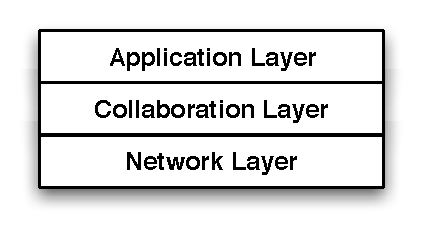
\includegraphics[width=6.6cm,height=3.42cm]{../images/layers.eps}
 \caption{The Layers of ACE}
\end{figure}

\paragraph{Application Layer:} The application layer consists mainly in the 
graphical user interface. The layer implementation in ACE is built with
Java Swing.

\paragraph{Collaboration Layer:} The collaboration layer provides the
collaborative editing functionality to the application layer. It hosts the core
consistency control algorithm, which is based on the concept of operational 
transformation. By replacing the collaboration layer it would be theoretically 
possible to replace the employed consistency control algorithm. Further it uses 
the network layer for all network related functionality.

\paragraph{Network Layer:} The network layer is the lowest layer of ACE. It 
provides networking functionality to the collaboration layer. The two most 
important features are discovery of users and documents as well as communication 
with other users and sessions. Replacing the network layer allows to use a 
different network technology and/or a different protocol.


%\section{Design Overview}
%The design of the different layers is based on interfaces. The packages
%\texttt{ch.iserver.ace.collaboration} and \texttt{ch.iserver.ace.net} contain
%the API of the layers.

\section{Interface between Collaboration and Application Layer}
The main class in the collaboration layer is the \texttt{CollaborationService}.
It is the entry point for an application layer. The main functionality 
exposed by the collaboration service are:
\begin{itemize}
 \item discovery of users and documents
 \item publishing of local documents
 \item registering invitation callback
\end{itemize}

\subsection{Discovery}
The collaboration service provides a listener registration mechanism for
users and documents. The corresponding methods are \texttt{addUserListener}
and \texttt{addDocumentListener}. These listeners are notified whenever a
new user or document are discovered by the underlying network layer.

The two listener interfaces are pretty similar. 
\begin{figure}[H]
 \centering
 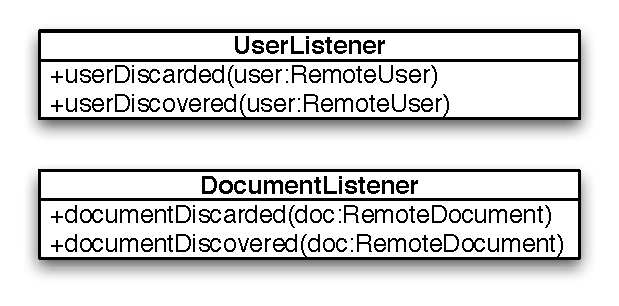
\includegraphics[width=9.9cm,height=4.6cm]{../images/design/discovery-listener.eps}
 \caption{DocumentListener and UserListener}
\end{figure}

The passed in objects are instances of \texttt{RemoteUser} and
\texttt{RemoteDocument} respectively. The user objects expose a \texttt{name}
property and documents expose a \texttt{title} property. Further, they support
property change events that are used to notify registered 
\texttt{PropertyChangeListener} instances about property value changes. The
\texttt{RemoteDocument} objects have also a property that returns the
\texttt{RemoteUser} for the publisher of the document.

\subsection{Joining Documents}
\texttt{RemoteDocument} instances have a method \texttt{join}. This join
method can be used to join a remote document. All that is needed to
join a document is to register a \texttt{DocumentListener} with the 
\texttt{CollaborationListener} and call join on a discovered document.

The \texttt{join} method is designed to return immediately. Join is a 
potentially long running operation. First, the join request has to be sent
to the publisher. Second, it might take some time to transfer the document
content over the network. And last but not least, if we ever implement
an access control mechanism, joining might need the approval of the publisher,
which might take even longer. Thus, it is a sensible design decision to
make this method non-blocking.

The result of join request is communicated to an object passed to the
\texttt{join} method implementing the \texttt{JoinCallback} interface.

\begin{figure}[H]
 \centering
 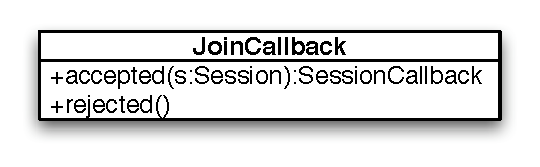
\includegraphics[width=8.5cm,height=2.25cm]{../images/design/collaboration-join.eps}
 \caption{JoinCallback interface}
\end{figure}

Depending on the outcome of the join request, either \texttt{accepted} or
\texttt{rejected} is called. The \texttt{accepted} method takes an argument
of type \texttt{Session} and returns a \texttt{SessionCallback}. The session
is the object that represents a collaborative editing session. It is
implemented by the collaboration layer and passed to the application layer.
The \texttt{SessionCallback} in turn is returned by the application layer
to the collaboration layer and is used by it to return received operations
and caret updates from other participants in the session.

\subsection{Publishing Documents}
To publish a document, the \texttt{CollaborationService} method \texttt{publish}
is used. The method has two parameters. The first is the session callback
for a published session. The second method is the \texttt{DocumentModel}
of the document to be published. The \texttt{DocumentModel} contains the
document content, the title, as well as the current caret position of the
publisher. The collaboration service in turn returns an object of type
\texttt{PublishedSession}, which is used both to control the session as well
as sending operations and updates to the caret position.

\subsection{Inviting Users}
\texttt{RemoteUser} instances have a method invite, which allows to invite
a user to a published session. The invite method is non-blocking, i.e. it
returns immediately. If the user accepts the invitation, he is added to the
list of participants of the session. Note: inviting users is not implemented.

\subsection{Listening for Invitations}
The \texttt{CollaborationService} has a method to register an
\texttt{InvitationCallback}. This callback is notified whenever another user
tries to invite the local user. 

\begin{figure}[H]
 \centering
 
\includegraphics[width=8.85cm,height=11.76cm]{../images/design/collaboration-invitationcallback.eps}
 \caption{InvitationCallback interface}
\end{figure}

The passed in \texttt{Invitation} allows to retrieve the document for which
the user is invited as well as the publisher of the document. However,
the important methods are \texttt{accept} and \texttt{reject}. They represent
the user actions of accepting or rejecting an invitation. Calling 
\texttt{accept} on the invitation returns the \texttt{Session} instance
for communicating with the session. A \texttt{SessionCallback} must be passed
in, which is used by the collaboration layer to notify the application
layer about events from the session.

\subsection{Communicating with a Session}
There are several ways to get a \texttt{Session} object:
\begin{itemize}
 \item joining a discovered remote document
 \item accepting an invitation
 \item publishing a local document (\texttt{PublishedSession})
\end{itemize}

All those ways have one thing in common: the pass a \texttt{SessionCallback}
(in case of publish a \texttt{PublishedSessionCallback}) to the collaboration
layer. There are always these two objects, a \texttt{Session} and
a \texttt{SessionCallback}. The \texttt{Session} is used by the application
layer to send events to collaboration layer and a \texttt{SessionCallback}
is used to notify the application layer about session related events from the 
collaboration layer. Figure \ref{fig:session and callback} depicts this 
situation.

\begin{figure}[H]
 \centering
 \includegraphics[width=10.37cm,height=7.02cm]{../images/design/collaboration-session.eps}
 \caption{Session and SessionCallback}
 \label{fig:session and callback}
\end{figure}

The \texttt{Session} interface has the following structure:

\begin{figure}[H]
 \centering
 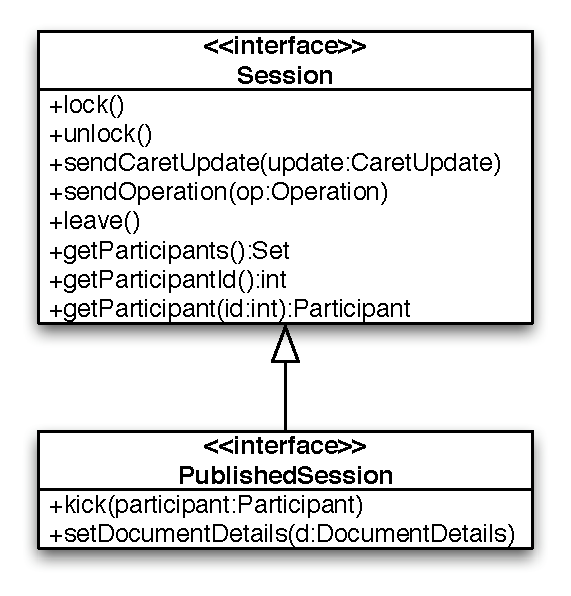
\includegraphics[width=9.1cm,height=9.53cm]{../images/design/collaboration-uml-session.eps}
 \caption{UML of Session and PublishedSession}
 \label{fig:session interface}
\end{figure}

Before anything can be sent to the session, it has to be locked. The method
\texttt{lock} is used to lock the session. For each lock call there must
be a corresponding \texttt{unlock} call, even in case of exceptions. Thus,
the unlock call should be placed inside a finally block to ensure proper
unlocking of the session.

Gaining the lock on the session must happen before the insertion index in
the document is determined. The lock ensures that either an operation/caret 
update from another participant or a local operation/caret update is processed
by the concurrency control algorithm. The locking is extremely important
to maintain the consistency of replicas.

The \texttt{sendXYZ} methods are used to send locally generated operations or
caret updates to the other participants in the session. The \texttt{leave}
method allows to leave the session, i.e. stop participating. The participant
related methods allow to access the currently participating users. These
methods return objects implementing the \texttt{Participant} interface. It has
two methods, one to get the \texttt{RemoteUser} and one to get the participant
id.

A participant id is a session-wide unique identifier for a user. They are given
to a user when he joins a session by the publisher of the session. The local
participant id can be retrieved by the \texttt{getParticipantId} method,
although this information is typically not used.

The interface used by the collaboration layer to notify the client of the
session about events is the \texttt{SessionCallback} interface.

\begin{figure}[H]
 \centering
 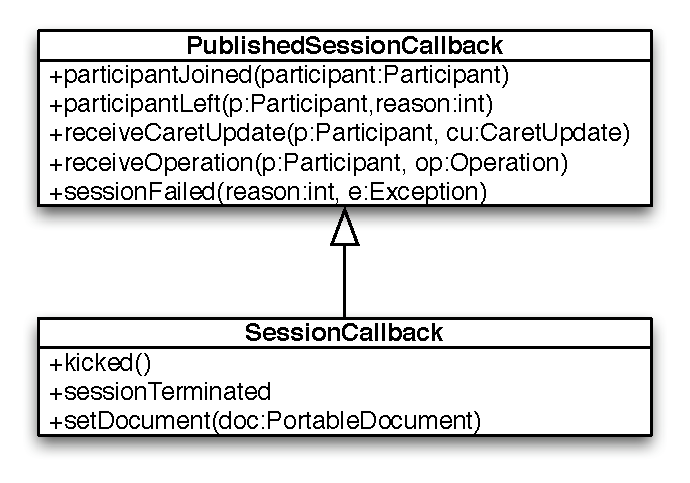
\includegraphics[width=11.11cm,height=7.62cm]{../images/design/collaboration-uml-sessioncallback.eps}
 \caption{UML of SessionCallback and PublishedSessionCallback}
 \label{fig:session callback interface}
\end{figure}

The inheritance in this case is different. A \texttt{PublishedSessionCallback}
is the superinterface of \texttt{SessionCallback} because it has fewer
methods. For instance, it is impossible that a publisher gets kicked from
the session.

The callback has methods to notify the client of the session about caret
updates and operations from other participants in the session. These methods
are named \texttt{receiveXYZ} and accept both a \texttt{Participant} object
as well as either an operation or a caret update.

The \texttt{participantXYZ} methods are used to notify the callback about
participants that joined or left the session. Finally, the session failed
method is used by the collaboration layer to notify the application layer
about a failed session. Reasons for this include failing network connection
to the publisher or unrecoverable situations in the collaboration or network
layer. The session should no longer be used after a call to 
\texttt{sessionFailed}.

The \texttt{SessionCallback} interface adds three additional methods. The
\texttt{kicked} method is used to notify the local user that he/she has
been kicked from the session by the publisher. The local user is no longer
welcome in that particular session. The \texttt{sessionTerminated} method
is called whenever the session has been concealed by the publisher. That
session no longer exists and the session object should no longer be used.
Finally, the \texttt{setDocument} method is used to pass the document
content to the application layer. This happens once, when the session is
joined.


\section{Interface between Collaboration and Network Layer}
In the last section we had a look at the interface between the application and
the collaboration layer. The collaboration layer itself cannot implement a
collaborative editor on itself. It needs a layer that provides the networking
functionality. The networking layer provides exactly that functionality to
the collaboration layer. It is not used directly by the application layer.

\subsection{Network Service}
The \texttt{NetworkService} interface is the entry point into the network layer.

\begin{figure}[H]
 \centering
 \includegraphics[width=11.11cm,height=7.62cm]{../images/design/network-uml-service.eps}
 \caption{UML of NetworkService}
 \label{fig:networkservice interface}
\end{figure}

\subsection{Network Service Callbacks}

